\subsubsection{Support Vector Machines}
	\label{svm}
	
	\paragraph{Background}
	The original Support Vector Machine (SVM) algorithm was formulated by Vladimir N. Vapnik and Alexey Ya. Chervonenkis in 1963 while working at the institute of Control Sciences in Moscow. Despite the theory behind SVMs being far from new today, it remained mostly theoretical until quite recently. The state of technology at the time of its conception was far behind the theory, and it would take decades until computers would reach the computational abilities that could facilitate SVMs.
	
	\paragraph{Implementation}
	SVM aims at segmenting an input dataset to binary categories (\cite{SVM_burges1998tutorial}). For example, positive and negative observations or analogously membership in or absence from a certain category. A common example is whether a given Email should be classified as Spam or not by the mail server. The rational behind SVMs could best be visualized by imposing the training observation on two dimensional Euclidean space. The algorithm strives to define a dividing line, which would create a separating threshold between the two groups. In two-dimensional space, the separator is demarcated using a simple line. Said line is then positioned in a manner, creating maximum separation between the two groups. This is achieved by drawing parallels through the closest positioned members of both groups. The linear divider lays in the middle between this two parallels. The observations which are positioned on the parallels themselves, define the \textit{curbs} of the so-called \textit{dividing street}, and are dubbed Support Vectors. From them in turn, the algorithm derives its name. Any new observation passed to the trained classifier for classification, will be allocated to the appropriate group, as is defined by its position relative to the separating hyperplane. 
	
	\begin{figure}[h]
		\centering
		\captionsetup{width=0.8\textwidth}
		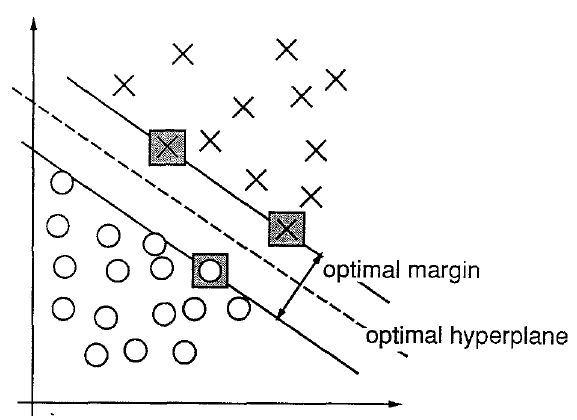
\includegraphics[width=0.8\textwidth]{svm.png}
		\caption[SVM in Euclidean Space]{
			\footnotesize{
				Euclidean Imposition of data. The support vectors, marked with grey squares, define the margin of largest separation between the two classes. \textit{Source:} \cite{SVM_cortes1995support}.
			}
		} 
	\end{figure}

 A dataset of size $n$ as in [\ref{svm_div_line}] is to be used as a training set, in which $y_i$ stands for the actual class of the observation $i$ and can have one of either values $y_i \in [+1;-1] $. The values represent a positive and negative classification accordingly. A positive $(+1)$ classification implies the presence of the sought-after class, $News$ in our case. The vector $(\textbf{x}_i)$ is an array of size $p$, representing the features which compose each observation. In the 2-dimensional example, the 2 features of $(\textbf{x}_i)$ can be graphically illustrated in euclidean space as the $(x,y)$ coordinates $(\textbf{x}_i) = [x_i^{(1)},x_i^{(2)}]$. 
	\begin{equation}
		\begin{aligned}
			(\textbf{x}_1,y_1),& ... , (\vec{x}_n,y_n), \ \ y \in \big[-1;+1 \big] \\
			\textbf{x}& = (x_{i1},x_{i2}, ...,x_{ip})
		\end{aligned}
	\label{svm_div_line}
	\end{equation}
	
	The optimal hyperplane segregates the two data classes, creating a maximally wide barrier between the closest observations of the opposing classes. This hyperplane is delineated in [\ref{svm_optimum}]. The vector $\vec{w}$ is the normal vector \footnote{A vector perpendicular to a given object, the diving hyperplane in this case} to the dividing hyperplane and the parameter $b$ represents the normal vector's offset along the axis. The area between the 2 hyperplanes, which pass through the closest observations is referred to as the \textit{margin} and is defined by the supporting vectors. These support vectors are illustrated in [\ref{svm_supp_vecs}].
	
	\begin{equation}
		\begin{aligned}
			\vec{w}& \cdot \textbf{x} - b = 0 \\
			\vec{w}& = (w_1, ... , w_p) 
		\end{aligned}
		\label{svm_optimum}
	\end{equation}
	
	\begin{equation}
		\vec{w} \cdot \textbf{x} - b = 
		\begin{cases}
			+1 \\
			-1 
		\end{cases}
		\label{svm_supp_vecs}
	\end{equation}
	
	The distance between any point and the separating line [\ref{svm_optimum}] is shown in equation [\ref{svm_dist}]. The distance between the 2 hyperplanes is equal to twice the distance between the support vectors and the separating line, hence $ \frac{2}{||\vec{w}||} $. The optimization problem at hand is thus the maximization of this distance, in order to create a maximally distinct margin between the classes. Furthermore, no observation from the training data can be positioned inside the margin [\ref{svm_constaints}].
	
	\begin{equation}
		\begin{aligned}
			\text{Dist.}&\text{ for point i}: \\ 
			&\frac{| \textbf{x}_i \cdot \vec{w} + b|}{||\vec{w}||},
		\end{aligned}
		\ \ \ \Rightarrow 	\ \ \ \ 
		\begin{aligned}
			\text{Dist.}&\text{ for support vectors:} \\
			&\frac{w^T\textbf{x} + b}{||\vec{w}||} = \frac{\pm 1}{||\vec{w}||}
		\end{aligned}
		\label{svm_dist}
	\end{equation}
	
	\begin{equation}
		\text{or}
		\begin{aligned}
			\vec{w}& \cdot \textbf{x} - b \geq 1 \ \ \forall \ \  y_i = +1 \\
			\vec{w}& \cdot \textbf{x} - b \leq 1 \ \ \forall \ \  y_i = -1
			\end{aligned}	
			\ \Rightarrow \ 
			\begin{aligned}
			y_i(&\vec{w} \cdot \textbf{x}_i - b) \geq 1 \\
			&\forall \ 1 \leq i \leq n
		\end{aligned}
		\label{svm_constaints}
	\end{equation}
	
	Finally, the core optimization problem is to enlarge the margin as much as possible, subject to all the training data points being located on the correct side of the margin, given their actual class. As denoted in [\ref{svm_opt_dist}].
	
	\begin{equation}
		\begin{aligned}
			&max \Bigg(\frac{2}{||w||}\Bigg) \Rightarrow 
			min \Bigg( \frac{w^Tw}{2}	\Bigg)\\
			&subject \  to \ \ y_i(\textbf{x}_i \cdot w + b) \geq 1
		\end{aligned}
		\label{svm_opt_dist}
	\end{equation}
	
	The optimal solution is array of values $\alpha$, which are the learned weights to the $x$'s and are equal zero for all but the support vectors ($y_i = \pm1 $). Incorporating the line [\ref{svm_div_line}] results in [\ref{svm_opt_dist2}].
	
	\begin{equation}
		w = \sum_{i=1}\alpha_i y_i \textbf{x}_i \ \ \ \xRightarrow[]{(\ref{svm_div_line})}
		\ \ \ w \cdot \textbf{x} + b = \textbf{x} \cdot  \sum_{i=1} \alpha_i y_i \textbf{x}_i  + b
		\label{svm_opt_dist2}
	\end{equation}
	
	It is now possible to derive a classification function based on the previous results. When classifying new data, unseen novel observations might fall inside the $[-1:+1]$ margin, and are therefore classified according their sign (positive/negative) as in equation [\ref{svm_sgn_function}].
	
	\begin{equation}
		f(x) = \text{sgn}(\vec{w} \cdot \textbf{x} + b)  =
		\text{sgn}\bigg( \sum_{i=1} \alpha_i
		\xunderbrace{
		 \xoverbrace{\textbf{x}_i}^{\substack{\text{New}\\ \text{Obs.}}}
	  \cdot 
	  \xoverbrace{\textbf{x}}^{\substack{\text{Support}\\ \text{Vectors}}}
		}_{dot \ product}
		 + b \bigg)
		\label{svm_sgn_function} 
	\end{equation}
	
	Notice that the results of the classification function depends solely on the dot product between the vector of the new point and the support vectors $(\textbf{x} \cdot\textbf{x}_i)$. It is hence possible to classify as shown in [\ref{svm_classification}].
	
	\begin{equation}
		\text{class}(x) = 
		\begin{cases}
			positive,\ \ \  &f(x) > 0 \\
			negative,\ \ \  &f(x) < 0
		\end{cases}
		\label{svm_classification}
	\end{equation}
	
	The basic SVM classification algorithm in itself seems to present a solution to a very limited spectrum of classification problems, that is two-dimensional, linearly-separable binary class classification problem. The following paragraph present solutions to each on of these difficulties. Notice that replacing the dot product from [\ref{svm_sgn_function}] can be generalized to any number $\mathbb{N}$ of dimensions, clearing the dimensionality restriction. The \textbf{Kernel Trick} resolves the linear-separability problem, by mapping to a higher dimension.
		
	\par		
	\paragraph{Kernel Trick}
	A key element of SVMs statistical and computational power is the Kernel Trick (\cite{guyon1993automatic}). Using the Kernel-Trick, the linearly dimensional training data $x$ are extrapolated onto a higher plane using a mapping function $\Phi:\textbf{x} \rightarrow \varphi(x)$, with the assumption that on the new plane a better linear separating hyper plane can be found. The mapping is carried out using a \textit{kernel trick}, where by the internal dot product of the linear separator is replaced with a Kernel Function. This Function simulates the redistribution of the original Support Vectors in a richer space, barely incurring an additional computational cost in the process. The linear separator in the new space is not bilinear on the original plane, thus the classification of new observation is also done using the Kernel Function. Whence the data is still not separable using a hyperplane in the new space, the dataset can be mapped to a higher still dimensional space. Mapping to a higher dimension is illustrated in equation [\ref{svm_phi_x}].
	
	\begin{figure}[h]
		\centering
		\captionsetup{width=0.8\textwidth}
		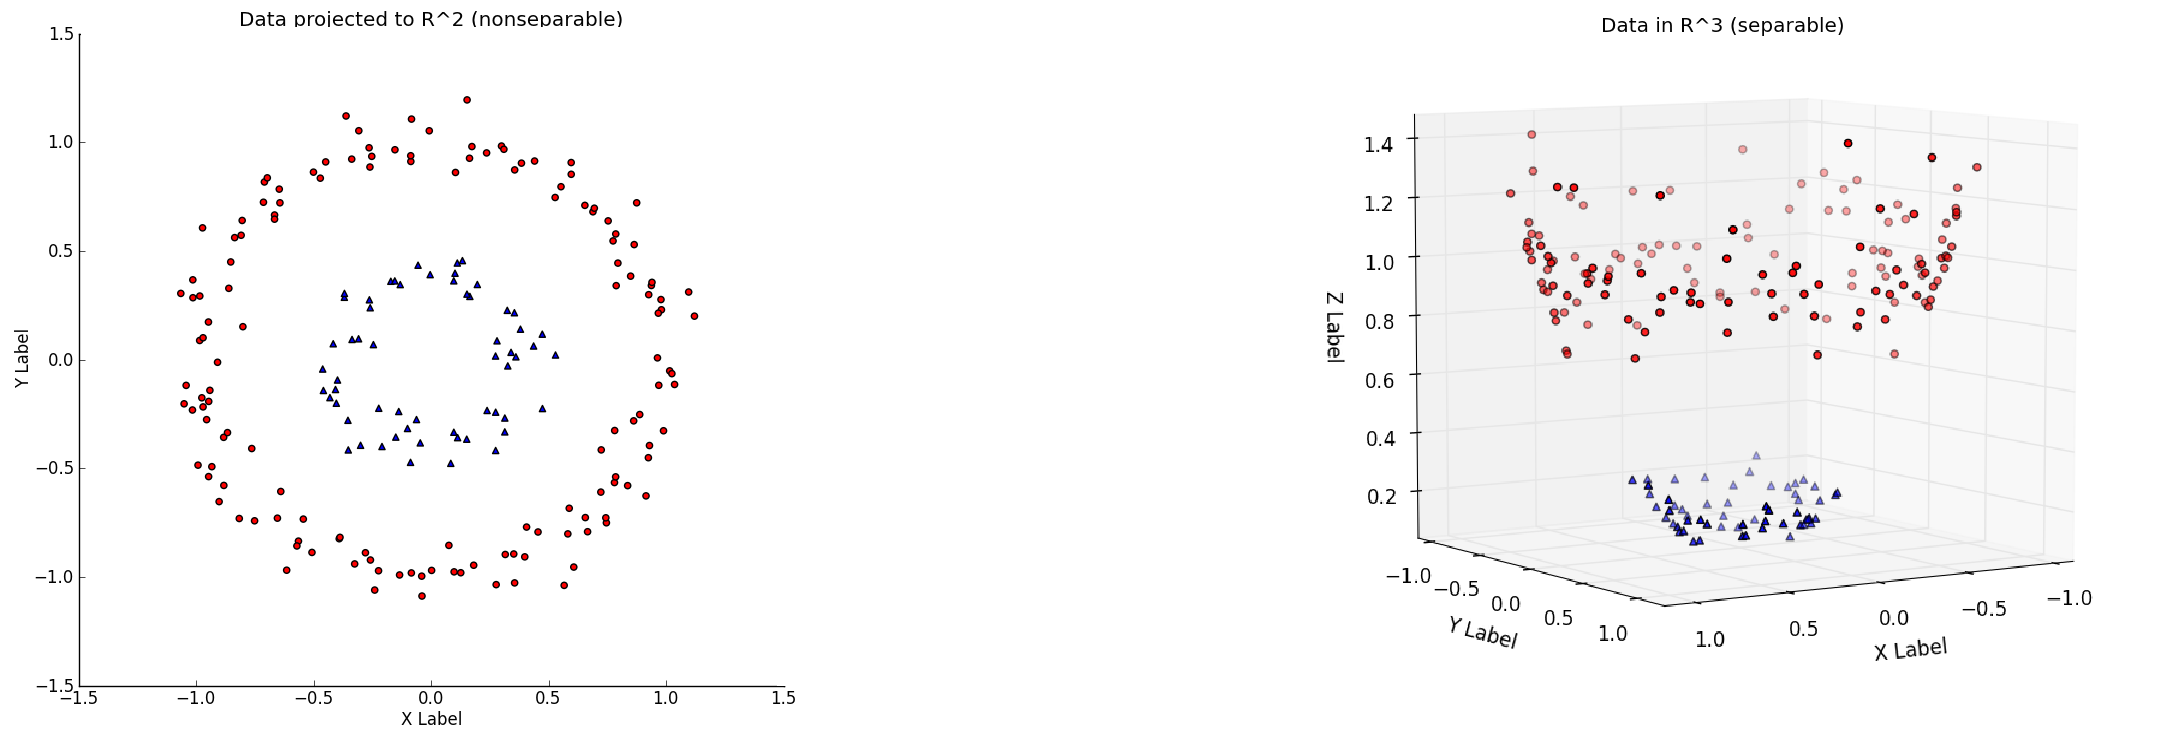
\includegraphics[width=0.8\textwidth]{data_2d_to_3d}
		\caption[SVM Dimensionianl Extrapolation]{
			\footnotesize{
				(Left) A dataset in  , not linearly separable. (Right) The same dataset transformed:
				$\varphi \big(x_1, x_2\big) \Rightarrow \big[ x_1,x_2,x_1^2+x_2^2 \big]$.
				\textit{Source}:\cite{kimso}
			}
		}
	\end{figure}

	\begin{equation}
		\begin{aligned}
			\mathlarger{\Phi}: \textbf{x} \ \ &\rightarrow \ \  \varphi(\textbf{x}) \\
			\mathlarger{K}(\textbf{x}) &\rightarrow \ \varphi(\textbf{x}_j)^T \varphi(\textbf{x}_j)
		\end{aligned}
		\label{svm_phi_x}
	\end{equation}
	
	\begin{equation}
		\sum_{i=1} \alpha_i y_i (\textbf{x}_i^T \textbf{x}) + b  \ \  \rightarrow \ \ 
		\sum_{i=1} \alpha_i y_i \mathlarger{K}(\textbf{x}_i, \textbf{x}) + b
		\label{svm_insert_kernel}
	\end{equation}
	
	The function K [\ref{svm_insert_kernel}] represents a \textit{kernel function} and acts as a similarity measure which corresponds to the inner product in some higher feature space. As long as there exists a dimensional space of greater magnitude, in which the kernel function is the dot product of that higher dimensional space, such a kernel is in fact a dot product, and as such can be classified using the normal linear classifier without loss of generality.
	
	\par	
\paragraph{Linear Kernel}
	The kernel is in simply the dot product [\ref{svm_lin_kernel}] and must not be mapped to a higher dimension. Therefore, the number of dimensions stays the same $ \mathbb{N} \rightarrow \mathbb{N} $.
	\begin{equation}
		\mathlarger{K}(x_i,x_j) = x_i^T x_j
		\label{svm_lin_kernel}
	\end{equation}

\paragraph{Polynomial Kernel}
	Training data is extrapolated using a polynomial kernel function [\ref{svm_poly_kernel_def}] into a higher dimensional space. The kernels represents the similarity of training samples in a feature space over polynomials of the original variables, allowing learning of non-linear models. Additionally, the polynomial kernel adds an interpretive intuition by applying interaction variables (products of $ x_i $ and $ x_j $).
	
	\begin{equation}
		\begin{aligned}
			\mathlarger{K}(\textbf{x}_i,\textbf{x}_j) = {(r + \gamma \cdot \textbf{x}_i^T \textbf{x}_j)}^d, \ \ \forall \gamma > 0 
		\end{aligned}
	\label{svm_poly_kernel_def}
	\end{equation}
	
	In [\ref{svm_poly_kernel_R2}] and [\ref{svm_poly_kernal_proof}] it is demonstrated that substituting the dot product with a kernel function results in the dot product on a higher dimension. Specifically [\ref{svm_poly_kernal_proof}] demonstrates the extrapolation of $ d=2 $ space to $ d=6 $ by employing a polynomial function.
	
	\begin{equation}
		\begin{aligned}
			&\text{Let   } \mathlarger{K}(\textbf{x}_i,\textbf{x}_j) = {(1 + \textbf{x}_i^T \textbf{x}_j)}^2 
			&\text{such that   } \textbf{x}: \mathbb{R}^2 \Rightarrow \mathbb{R}^6
		\end{aligned}
		\label{svm_poly_kernel_R2}
	\end{equation}
	
	\begin{equation}
		\begin{split}
			\mathlarger{K} \xoverbrace{(\textbf{x}_i,\textbf{x}_j)}^{\mathbb{R}^2}
			&= {(1 + \textbf{x}_i^T \textbf{x}_j)}^2 \\
			& = 1+ x_{i1}^2 x_{j1}^2 
			+ 2 \big(x_{i1}x_{j1} +  x_{i1}x_{j1}x_{i2}x_{j2} + x_{i2}x_{j2}\big) 
			+ x_{i2}^2 x_{j2}^2 \\ 
			& = \big[
				1 + x_{i1}^2 + \sqrt{2}x_{i1}x_{i2} + x_{i2}^2 + \sqrt{2}x_{i1} + \sqrt{2}x_{i2}
			\big]^T
			\cdot \\
			&\hspace{2cm} \big[
				\underbrace{1 + x_{j1}^2 + \sqrt{2}x_{j1}x_{j2} + x_{j2}^2 + \sqrt{2}x_{j1} + \sqrt{2}x_{j2}}_{\mathbb{R}^6}
			\big] \\
			&= \varphi(x_i)^T\varphi(x_j) \\ 
			\text{such that :}&\\
			 \varphi(x) &= \big[
				 \xoverbrace{1 + x_1^2  + \sqrt{2}(x_1 + x_1x_2 + x_2) + x_2^2}^{\mathbb{R}^6}
			 \big]
		\end{split}
		\raisetag{2\normalbaselineskip}
		\label{svm_poly_kernal_proof}
	\end{equation}
	
\paragraph{Gaussian Radial Basis Kernel}
	The Radial Basis Function (RBF) is a prevalent kernel in Machine Learning algorithms.
	\begin{equation}
		 \begin{aligned}
			\mathlarger{K}(\textbf{x}_i,\textbf{x}_j) = \mathlarger{\mathlarger{e}}^{
				\displaystyle  -\Bigg(
				\frac{||\textbf{x}_i - \textbf{x}_j||^2}{2 \sigma^2}
				\Bigg)}& \ \ \
			\overset{\mathclap{\tikz \node {$\downarrow$} node [above=1ex] {$\gamma = \frac{1}{2\sigma^2}$};}}{=}
			\mathlarger{\mathlarger{e}}^{\displaystyle  -\big(
				\gamma \cdot ||\textbf{x}_i - \textbf{x}_j||^2
				\big)}, \\
			& \forall \gamma \ > 0 
		 \end{aligned}
	\end{equation}
	The RBF kernel ranges between zero (in the limit) and one (when $\textbf{x}_i = \textbf{x}_j$) and declines as the distance between the points grows smaller. RBF is likewise interpreted as a similarity measure, which is why it converges well to the kernel function idea. The feature space of the kernel is of infinite dimensionality.
	
\paragraph{Sigmoid Kernel}
	The Sigmoid function, also known as the Hyperbolic Tangent function, bares semblance to the behavior of the logistic regression by creating an "S"-shaped curve. 
	
	\begin{figure}[h]
		\centering
		\captionsetup{width=0.8\textwidth}
		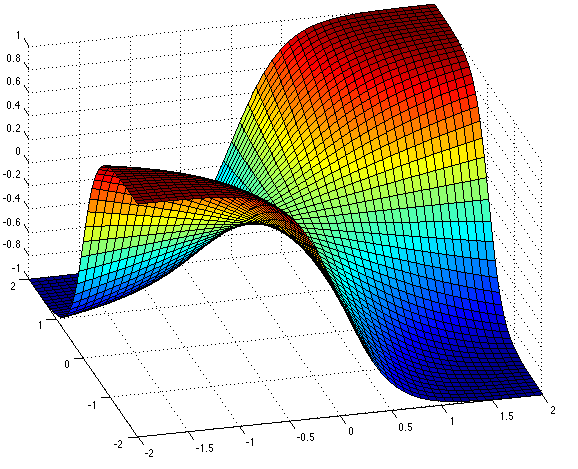
\includegraphics[width=0.5\textwidth]{sigmoid}
		\caption[Sigmoid Kernel]{
			\footnotesize{
				Sigmoid Kernel visualization in d = 3. \textit{Source:} \cite{carrington2014new}
			}
		}
	\end{figure}
	
	This kernel originates from Neural Networks, another Machine Learning algorithm. The kernel, when implemented, produces an SVM equivalent to a two-layer Perceptron Neural Network.
	\begin{equation}
		\mathlarger{K}(\textbf{x}_i,\textbf{x}_j) = \text{tanh}(\gamma \cdot \textbf{x}^T_i \textbf{x}_j + r)
	\end{equation}
	


\paragraph{Margin Rigidity or Slack}
	Current research of SVM usage revolves around the concept of \textit{Soft-Margins} (\cite{SVM_cortes1995support}). In the case of not linearly separable data, which is usually the case, a \textit{hinge loss} function is added to formula. Its purpose is to penalize for observations, which are on the 'wrong' side of the margin, that is between the 'sidewalk' and 'separator'. Using this method, observation are allowed to break the constraint present in the hard-margin case [\ref{svm_opt_dist}]. In other words, observations are permitted to cross to the "wrong side" of the margin, but they are being penalized for it, as demonstrated through the variable $c$ in [\ref{svm_soft_margin}]. A trade-off between margin width, which represents the distinctness of each class, and the amount of misclassified observations can than be specified by the user.

	\begin{equation}
		\begin{aligned}
			max \ (c - y_i(\vec{w} \cdot \textbf{x}_i - b)), 
			\  \ \ \forall \ c = \ 
			\begin{cases} 
				0 \ \ \text{if} \ (8) \ \text{holds true}\\
				1 \ \ \text{else}
			\end{cases}
		\end{aligned}
		\label{svm_soft_margin}
	\end{equation}

	The optimization problem with the soft-margins approach is represented in Equation [\ref{svm_sof_marg_opt}]. The variable $\lambda$ controls the penalty magnitude for observations being on the wrong side of the margin. $\lambda$ therefore, represents the trade off between margin size and the observation being correctly classified. As the $\lambda$ approaches zero, the problem converges into the hard margin scenario.

	\begin{equation}
		\Bigg[
		\frac{1}{n} \sum_{i=1}^{n}max(c-y_i(\vec{w} \cdot \textbf{x}_i - b )) 
		\Bigg]
		+ \lambda || \vec{w} ||^2
		\label{svm_sof_marg_opt}
	\end{equation}

\paragraph{Multiclass classification}
	The classification model in itself is natively used for binary stratification, that is 2 classes only. However, as may be the case in many classification scenarios, data has more then 2 dimensions. For the purpose of Multiclass classification using SVMs, a process known as \textit{class-reduction} is implemented (\cite{aly2005survey}). This is done by either a 'one-vs-all' or 'one-vs-one' approach. With the former method, classifiers for each given class $c$ are trained to differentiate it from the rest of the set. The testing data is then inputed into each of the classifiers and the highest scoring one (having the largest distance from the decision boundary) determines the class for each observation. This is also known as the \textit{winner-takes-all} approach. Using the latter method consists of training classifiers for every combination of two classes out of all the classes. In the case where there are $n$ classes, $\frac{n(n-1)}{2} $ classifiers will be trained as in [\ref{one_v_one}]
	a max-wins voting strategy, whereby every observations is denoted to one of two classes by each classifier. Afterwards, the final classification is determined by a tally of the votes on each new data point.
	
	\begin{equation}
		\begin{aligned}
			\text{Classes:}	\ \ \ \ \ \ \ \	\textbf{c} &= (c_1,c_2,c_3,c_4) \\
			\text{Classifiers:}\ \ \ 	\textbf{Cl.} &= (Cl_{12},Cl_{13},Cl_{14},Cl_{23},Cl_{24},Cl_{34})
		\end{aligned}	
		\label{one_v_one}
	\end{equation}

\paragraph{Strengths and Weaknesses}
	Among the advantages of SVMs one can mentions several factors. Firstly, the usage of different kernels - especially user-specified ones, allows for expert knowledge to be integrated into the classification problem. Secondly, the optimization space for the categorization problem is convex, thus making it easily and usually swiftly solvable with appropriate solving algorithms. And thirdly, the usage of soft-margins, or penalizing for error in classification makes the user more aware of the imminent over-fitting, which is the bane of classification problems. This awareness encourages the user to take a more cautious approach and avoid over-specification. The disadvantages include but are not limited to the following. The choice of kernel is for the user to decide, which could add to the element of human error, especially with dilettante users. Secondly, the problem of Multiclass classification is not solved directly, but rather is adopted for, by creating a multitude of partial SVMs, making it not the most effective tool for such scenarios. Finally, the algorithm tends to be memory intensive during the training phase. Because a value needs to be calculated for each pair of $n$ points, a matrix of size $n^2$ must be constructed. For example, when training with a dataset of size $n = 1,000$ - the kernel values matrix will be $n^2 = 1,000,000$ large. In optimized modules though, you can get away with only calculating half of the matrix, since its symmetrical along its diagonal.
